\documentclass[11pt,a4paper]{article}
\usepackage[utf8]{inputenc}
\usepackage[T1]{fontenc}
\usepackage{amsmath,amssymb,amsthm}
\usepackage{booktabs,array,calc}
\usepackage{tabularx}
\usepackage{graphicx}
\usepackage{geometry}
\geometry{margin=1in}
\usepackage{microtype}
\usepackage{soul}
\usepackage{caption}
\usepackage{algorithm}
\usepackage{algpseudocode}
\usepackage{cite}
\usepackage{hyperref}
\hypersetup{
    colorlinks=true,
    linkcolor=blue,
    citecolor=blue,
    urlcolor=blue
}

\newtheorem{definition}{Definition}
\newtheorem{condition}{Condition}
\newtheorem{proposition}{Proposition}

\title{\textbf{Prediction-Informed Selective Route Resequencing for Dispatch Service-Threshold Lateness Mitigation under Limited Intervention Capacity}}
\author{}
\date{}

\begin{document}

\maketitle

\begin{abstract}
\noindent
\textbf{Keywords:} Last-mile delivery; Delivery lateness prediction; Prediction-informed decision making; Route resequencing; Service reliability
\end{abstract}

\section{Introduction}\label{sec:introduction}

The continued expansion of e-commerce has increased both the scale and
service expectations of last-mile delivery operations. Customers
increasingly evaluate delivery performance not only by whether an order
is successfully delivered but also by whether it arrives within the
dispatch service threshold. Maintaining such reliability is challenging because
last-mile operations involve geographically dispersed customers,
fluctuating workloads, and substantial operational uncertainty. Delivery
lateness can therefore remain a persistent service problem even in
established delivery networks, creating a need for operational
mechanisms that can identify at-risk deliveries and respond before
service failures occur. The growing availability of operational delivery
data provides an opportunity to address this challenge through
predictive analytics. Information on orders, dispatch service thresholds,
locations, courier assignments, and historical outcomes can be used to
identify patterns associated with delivery failures. Recent studies have
consequently applied machine-learning methods to delivery-delay
prediction, arrival-time estimation, and service-completion prediction
\cite{pegado2023,zhang2024,muller2025}.
However, identifying deliveries that are likely to be late does not by
itself determine how operators should respond to them.

This distinction between prediction and operational action is
increasingly recognized in prescriptive analytics. Predictive models are
generally evaluated according to statistical accuracy, whereas their
practical value ultimately depends on the downstream decisions they
support. Better predictive performance does not necessarily translate
into better operational outcomes \cite{elmachtoub2022,yan2022,wang2023}.
Transportation research has therefore
increasingly integrated learned information with routing and related
operational decisions, including data-driven last-mile routing
\cite{dieter2023,ghosh2023,ozarik2024}, inventory routing
\cite{jia2025}, and vehicle rebalancing \cite{guo2026}.
These developments suggest that delivery-risk predictions should be
evaluated not only by how accurately they identify potential failures
but also by whether they lead to useful operational interventions. This
prediction-to-intervention problem is particularly relevant when route
adjustments are costly or operationally limited. If only a subset of
deliveries can be prioritized for adjustment, selecting customers solely
according to predicted lateness risk may not be sufficient. A delivery
with high predicted risk may offer little opportunity for improvement
through a feasible route change, whereas another delivery may be easier
to advance with limited disruption to the existing route. Effective
intervention targeting should therefore consider both lateness risk,
representing the need for intervention, and actionability, representing
the opportunity for a feasible intervention to improve the outcome.
Moreover, moving a customer within a delivery sequence can alter the
arrival times of downstream customers and increase route distance. The
effectiveness of an intervention must consequently be assessed at the
route level rather than inferred simply from whether a high-risk
customer was targeted.

Existing research provides substantial foundations for delivery-outcome
prediction, prediction-informed transportation decisions, and
service-oriented route adjustment
\cite{florio2018,pegado2023,dieter2023,ozarik2024}. Nevertheless,
comparatively limited attention has been devoted to connecting ex-ante
customer-level service-threshold lateness prediction with selective route
resequencing under constrained intervention capacity, particularly when
intervention priorities reflect both predicted risk and actionability
and the resulting service improvements are evaluated against additional
routing effort. Addressing this intersection requires moving beyond the
question of which deliveries are likely to be late toward determining
which predicted risks warrant intervention and whether the resulting
route adjustments produce meaningful service improvements. We refer to
this decision problem as the Dispatch Service-Threshold Delivery Lateness Mitigation
Problem (PTDLMP) and develop a Prediction-Informed Selective Route
Resequencing (PISR) framework to address it. PISR first estimates
customer-level service-threshold lateness risk using only information
available before the delivery outcome is realized. The predicted risk is
then combined with intervention actionability to prioritize candidate
deliveries. Selected customers are moved forward within an existing
delivery sequence subject to an intervention budget and a route-distance
tolerance. Counterfactual time propagation is subsequently used to
evaluate how the modified route affects late deliveries and tardiness,
together with the additional routing effort required. Accordingly, this
study addresses three research questions:

\hl{\textbf{RQ1.} How reliably can customer-level dispatch service-threshold delivery
lateness be predicted using only information available before delivery?}

\hl{\textbf{RQ2.} Can predicted lateness risk improve the selection of
deliveries for route intervention relative to risk-unaware targeting
strategies under limited intervention capacity?}

\hl{\textbf{RQ3.} To what extent can selective prediction-informed route
resequencing reduce simulated late deliveries and tardiness, and what
additional routing effort is required to achieve these improvements?}

This study makes three contributions. \hl{First, it establishes a
leakage-free customer-level prediction setting for dispatch service-threshold
delivery lateness using chronological model development and evaluation,
thereby aligning risk estimation with the information available before
intervention. Second, it develops a selective intervention approach that
distinguishes lateness risk from intervention actionability and compares
risk-based, actionability-based, and combined risk--actionability
targeting under explicit intervention budgets. Third, it evaluates
predictions through their downstream operational consequences using
counterfactual route simulation, quantifying reductions in late
deliveries and tardiness against additional routing effort and examining
whether stronger predictive performance translates into better
intervention outcomes.} The remainder of this paper is organized as
follows. Section 2 reviews delivery lateness prediction,
prediction-informed logistics decisions, and service-oriented route
adjustment. Section 3 defines the PTDLMP and presents the PISR
framework. Section 4 describes the data, predictive methodology, route
construction, experimental design, performance measures, and statistical
analysis. Section 5 presents and discusses the predictive and
operational results, including prediction-to-decision, ablation, and
robustness analyses. Section 6 concludes with the main findings,
implications, limitations, and future research directions.

\section{Literature Review}\label{sec:literature-review}

This section reviews three streams of research that underpin the
proposed study: delivery lateness prediction, prediction-informed
decision making in logistics, and route adjustment for improving
last-mile service reliability. Together, these streams establish the
methodological foundations for predicting delivery outcomes and
incorporating data-driven information into operational decisions, while
also revealing the need for closer integration between customer-level
lateness prediction and selective route intervention.

\subsection{Delivery lateness prediction in e-commerce and last-mile logistics}\label{sec:lit-prediction}

Delivery reliability has become an important concern in e-commerce and
last-mile logistics because deviations from dispatch service thresholds can
directly affect customer experience and service performance. The
increasing availability of operational data has consequently motivated
the use of predictive analytics to anticipate delivery delays and
related service outcomes. Müller et al. \cite{muller2025}, in a systematic review
of predictive methods for supply-chain delivery delays, document the
growing use of machine-learning approaches for delay prediction and
highlight the importance of moving beyond predictive accuracy toward
operationally useful predictions. Related research has examined more
specific delivery outcomes, including estimated arrival times, service
completion, and route execution. For example, Zhang et al. \cite{zhang2024}
developed a heterogeneous hypergraph neural network for package
arrival-time estimation by capturing complex relationships among
delivery-related entities. Pegado-Bardayo et al. \cite{pegado2023} proposed a
data-driven decision-support system that combines machine-learning
prediction with route-pattern information to anticipate service
completion in last-mile operations. Such studies demonstrate that
operational data can provide useful signals about future delivery
outcomes before service execution is completed.

An important methodological consideration, however, is the timing of
prediction. A prediction intended to support an operational intervention
should rely only on information available when that intervention can
actually be made. Features generated after route execution, delivery
completion, or the realization of the outcome may improve apparent
predictive performance but cannot support a genuine ex-ante decision.
This distinction is particularly important for dispatch service-threshold
performance, where the operational value of a prediction depends not
only on whether lateness can be identified accurately but also on
whether the risk is identified early enough to support corrective
action. Accordingly, the present study focuses on customer-level
service-threshold lateness prediction using a leakage-free information set
and chronological model development and evaluation.

\subsection{Prediction-informed decision making in logistics}\label{sec:lit-decision-making}

Accurate prediction does not necessarily translate into better
operational decisions. This distinction has received increasing
attention in prescriptive analytics and predict-then-optimize research.
Elmachtoub and Grigas \cite{elmachtoub2022} show that minimizing conventional
prediction error can be misaligned with the quality of downstream
optimization decisions, motivating learning approaches that explicitly
account for decision consequences. In transportation, Yan and Wang
\cite{yan2022} review the integration of prediction and optimization and
emphasize the value of connecting predictive information with
operational decision models. Similarly, Soeffker et al. \cite{soeffker2022} frame
stochastic dynamic vehicle routing from a prescriptive-analytics
perspective in which information models and decision models interact,
while Wang and Yan \cite{wang2023} discuss methodological challenges in
evaluating prediction-supported freight transportation decisions. Recent
studies demonstrate several ways in which learned information can
influence transportation decisions. Dieter et al. \cite{dieter2023} integrate
machine learning and routing optimization to incorporate driver behavior
into last-mile route planning. Özarık et al. \cite{ozarik2024} use machine learning
to evaluate candidate delivery sequences and combine these predictions
with classical routing procedures to improve last-mile route selection.
Ghosh et al. \cite{ghosh2023} combine globally learned historical routing
information with local optimization to generate delivery routes that
better reflect operational routing practices. Mo et al. \cite{mo2023} use a
pair-wise attention-based pointer neural network to predict
drivers' route trajectories, while Canoy et al. \cite{canoy2024}
investigate probability estimation and structured-output prediction for
learning routing preferences in last-mile delivery.

The prediction-to-decision perspective also extends beyond conventional
last-mile routing. Jia et al. \cite{jia2025} develop a scenario
predict-then-optimize framework in which predicted future demand
supports online inventory-routing decisions. More recently, Guo et al.
\cite{guo2026} propose a smart predict-then-optimize framework for vehicle
rebalancing and further demonstrate the potential mismatch between
predictive loss and downstream decision quality. Hu et al. \cite{hu2026}
similarly integrate individual risk prediction with selection and
routing decisions in an inspection setting, illustrating how
entity-level risk information can be translated into operational
prioritization under resource constraints. These developments are
particularly relevant when intervention resources are limited. In such
settings, identifying which entities are most likely to experience an
undesirable outcome is only one part of the decision problem. A high
predicted risk does not necessarily imply that an operational
intervention can effectively alter the outcome. Conversely, an easily
adjustable delivery may provide little benefit if it is unlikely to be
late. This distinction motivates separating risk, which represents the
need for intervention, from actionability, which represents the
opportunity for an intervention to improve the outcome. The operational
value of prediction should therefore be assessed not only through
predictive performance but also through the quality of the decisions and
outcomes generated from those predictions.

\subsection{Route adjustment and service reliability in last-mile delivery}\label{sec:lit-route-adjustment}

Vehicle-routing research provides an extensive foundation for adapting
routes in response to operational information and service requirements.
Pillac et al. \cite{pillac2013} review dynamic vehicle-routing problems in which
routes may be revised as new information becomes available, while Zhang
and Van Woensel \cite{zhang2023} provide a more recent review of dynamic vehicle
routing with random requests and highlight the growing role of
information in routing decisions. These studies establish route
adjustment as an important mechanism for responding to changing
operational conditions. Within last-mile delivery, routing decisions
increasingly incorporate considerations beyond transportation cost
alone. Florio et al. \cite{florio2018}, for example, optimize e-commerce delivery
routes using customer availability profiles and demonstrate the
trade-off between successful delivery performance and transportation
cost. Cook et al. \cite{cook2024} develop constrained local-search procedures for
last-mile routing that account for operational characteristics derived
from real delivery environments. Ji et al. \cite{ji2022} study on-site service
scheduling and routing with the objective of reducing the risk of
missing appointment times and show how service-risk considerations can
influence routing and re-optimization decisions. Collectively, these
studies illustrate that customer service considerations, operational
information, and routing efficiency can be incorporated jointly into
route-planning decisions. The intervention setting considered in this
study differs from constructing or fully re-optimizing a route from
scratch. When a baseline route already exists and only limited
operational adjustments are feasible, the decision becomes one of
selective route intervention: which deliveries should receive priority
for adjustment, how should their route positions be modified, and
whether the resulting service improvement justifies the associated
routing burden. This setting also requires intervention effects to be
evaluated at the route level. Moving one customer forward in a sequence
changes not only that customer\'s arrival time but
potentially the arrival times of downstream customers. Consequently,
intervention effectiveness cannot be inferred simply from the number of
targeted customers; it should be evaluated by propagating the modified
route schedule and measuring the resulting changes in lateness,
tardiness, and routing effort.

Prior researches provide substantial foundations for delivery-outcome
prediction, prediction-informed transportation decisions, and
service-oriented route adjustment. At the same time, comparatively
limited attention has been devoted to linking ex-ante customer-level
service-threshold lateness risk with selective route resequencing under
constrained intervention capacity, while explicitly considering both the
actionability of potential interventions and their downstream
route-level consequences. The present study addresses this intersection
by examining how predicted service-threshold lateness risk can be combined
with intervention actionability to prioritize a limited set of
deliveries for route resequencing and by evaluating whether the
resulting service improvements justify the additional routing effort.
This prediction-to-intervention perspective provides the basis for the
dispatch service-threshold lateness mitigation problem and the framework
developed in the following section.

\section{Prediction-Informed Selective Route Resequencing (PISR) Framework}\label{sec:pisr-framework}

\subsection{Problem definition and decision setting}\label{sec:problem-definition}

Consider a last-mile delivery setting in which a set of customer orders
is assigned to a courier for service within a delivery day. Each order
is associated with a dispatch service threshold, and the operational problem
is to identify deliveries at risk of service-threshold lateness and
determine whether selectively changing their service positions can
improve route-level service performance. Intervention is subject to
limited operational capacity and a constraint on the allowable increase
in route distance. The intervention decision is made before delivery
outcomes are realized. At this decision epoch, order characteristics,
service-threshold information, customer locations, planned workload, and
strictly historical performance information may be available. In
contrast, realized delivery timestamps, realized customer service
sequences, and other post-execution outcomes are unavailable and cannot
be used for risk estimation or intervention decisions. This ex-ante
information boundary defines the decision setting considered throughout
this study.

Let \(C = \left\{ 1,\ldots,n \right\}\) denote the set of customers
assigned to a courier-day route and let
\(R = \left( i_{1},i_{2},\ldots,i_{n} \right)\) denote a service
sequence containing each assigned customer exactly once. For customer
\(i\), let \(\tau_{i}\) denote the dispatch service threshold and
\(a_{i}(R)\) the route-propagated service time under route \(R\).

\begin{definition}[Service-threshold lateness] Customer \(i\) is late
under route \(R\) when its route-propagated service time exceeds its
dispatch service threshold:

\begin{equation}
L_{i}(R) = \left\{ \begin{matrix}
1, & a_{i}(R) > \tau_{i}, \\
0, & \text{otherwise}.
\end{matrix} \right.\
\label{eq:1}
\end{equation}

The corresponding tardiness is

\begin{equation}
T_{i}(R) = \max\left\{ 0,a_{i}(R) - \tau_{i} \right\}.
\label{eq:2}
\end{equation}

The number of late deliveries and total tardiness under route \(R\) are
respectively

\begin{equation}
NL(R) = \sum_{i \in C}^{}L_{i}(R),
\label{eq:3}
\end{equation}

and

\begin{equation}
TT(R) = \sum_{i \in C}^{}T_{i}(R).
\label{eq:4}
\end{equation}
\end{definition}

Historical observations used for predictive learning are distinguished
from customers in the operational intervention problem. Let \(h\) index
a historical order observation, \(d_{h}\) denote its realized delivery
time, \(y_{h}\) its observed service-threshold lateness label, and \(x_{h}\)
the information vector available before its delivery execution. These
historical observations are used to learn the relationship between
ex-ante order information and service-threshold lateness. For customer
\(i\) in the operational intervention setting, the corresponding ex-ante
information vector \(x_{i}\) is subsequently used to estimate
customer-level lateness risk. Let \(R^{0}\) denote an ex-ante baseline
service sequence for customer set \(C\), and let \(R'\) denote a
modified sequence after intervention. Both routes contain the same
customer set; intervention changes only service positions and does not
remove customers or reassign them across couriers.

The resulting decision problem is referred to as the Dispatch Service-Threshold
Delivery Lateness Mitigation Problem (PTDLMP). Given an assigned
customer set, an ex-ante baseline route, customer-level lateness-risk
information, limited intervention capacity, and an allowable
route-distance increase, PTDLMP concerns which deliveries should be
prioritized for intervention and whether feasible route resequencing can
mitigate service-threshold lateness and tardiness without excessive
additional routing effort. The proposed approach for addressing PTDLMP
is introduced in Section 3.2.

\begin{table}[htbp]
\centering
\caption{Used notations in the proposed method}
\label{tab:notations}
\small
\setlength{\tabcolsep}{4pt}
\renewcommand{\arraystretch}{1.12}
\begin{tabularx}{\textwidth}{@{}l>{\raggedright\arraybackslash}Xl>{\raggedright\arraybackslash}X@{}}
\toprule
\textbf{Symbol} & \textbf{Definition} & \textbf{Symbol} & \textbf{Definition} \\
\midrule
$C$ & Set of customers assigned to a route, indexed by $i$ & $T_{i}(R)$ & Tardiness of customer $i$ under route $R$ \\
$n$ & Number of customers & $NL(R)$ & Number of late deliveries under route $R$ \\
$r$ & Courier-day route index & $TT(R)$ & Total route tardiness under route $R$ \\
$n_{r}$ & Number of customers assigned to courier-day route $r$ & $p_{i}$ & Predicted service-threshold lateness probability of customer $i$ \\
$R$ & Generic customer service sequence & $g_{i}$ & Intervention actionability score of customer $i$ \\
$R^{0}$ & Ex-ante baseline customer service sequence & $\Delta TT_{ij}$ & Potential reduction in baseline total tardiness from relocating customer $i$ to position $j$ \\
$R^{c}$ & Current customer service sequence during sequential intervention & $F_{i}$ & Set of feasible forward positions for customer $i$ under the actionability assessment \\
$R'$ & Final customer service sequence after intervention & $J_{i}$ & Set of candidate forward positions for customer $i$ \\
$R^{0,i \rightarrow j}$ & Route obtained by relocating customer $i$ from its position in baseline route $R^{0}$ to position $j$ & $S_{i}^{RB}$ & Risk-Based targeting score of customer $i$ \\
$R^{c,i \rightarrow j}$ & Route obtained by relocating customer $i$ from its position in route $R^{c}$ to position $j$ & $S_{i}^{AB}$ & Actionability-Based targeting score of customer $i$ \\
$i_{k}$ & Customer occupying position $k$ in a service sequence & $RAS_{i}$ & Risk-Actionability score of customer $i$ \\
$j$ & Candidate insertion position for a forward relocation & $B$ & Intervention-budget proportion \\
$k$ & Current position of the selected customer in a service sequence & $K_{r}(B)$ & Maximum number of customers admitted for intervention on route $r$ under budget $B$ \\
$\tau_{i}$ & Dispatch service threshold of customer $i$ & $C_{r}^{B}$ & Set of customers admitted for intervention on route $r$ under budget $B$ \\
$d_{h}$ & Realized delivery time of historical order $h$ & $\delta$ & Maximum allowable relative increase in route distance \\
$y_{h}$ & Observed service-threshold lateness label of historical order $h$ & $D(R)$ & Total route distance $R$ \\
$x_{i}$ & Ex-ante predictor vector of customer $i$ & $\Delta NL$ & Change in number of late deliveries between baseline route $R^{0}$ and final route $R'$ \\
$a_{i}(R)$ & Route-propagated service time of customer $i$ under route $R$ & $\Delta TT$ & Reduction in total tardiness between baseline route $R^{0}$ and final route $R'$ \\
$L_{i}(R)$ & Service-threshold lateness indicator of customer $i$ under route $R$ & $\Delta D$ & Relative change in route distance between baseline route $R^{0}$ and final route $R'$ \\
\bottomrule
\end{tabularx}
\end{table}

\subsection{Framework architecture and decision flow}\label{sec:framework-architecture}

To address PTDLMP, this study proposes a PISR framework that links
ex-ante lateness-risk prediction with targeted route intervention. As
illustrated in Fig. 1, the framework comprises five connected
components: (i) ex-ante customer-level lateness-risk estimation, (ii)
ex-ante baseline-route construction, (iii) risk- and
actionability-informed intervention prioritization, (iv) selective
forward relocation, and (v) counterfactual route-outcome evaluation. The
prediction component estimates customer-level lateness risk before route
execution, while the baseline-route component establishes the service
sequence against which intervention opportunities are assessed.
Predicted risk and route-based actionability are then used to prioritize
customers under limited intervention capacity. Selected customers are
considered sequentially for forward relocation subject to routing
feasibility and strict tardiness improvement. Finally, the modified
route is evaluated through counterfactual time propagation to quantify
changes in service-threshold violations, total tardiness, and routing
effort. A central feature of PISR is the separation between prediction,
targeting, and route modification. Predicted lateness risk informs which
customers warrant greater intervention priority but does not directly
determine whether or where a customer is relocated. Likewise, selection
for intervention does not imply that a feasible beneficial relocation
exists. Actual route modification is determined by the constrained
relocation procedure developed in Section 3.6.

\begin{figure}[htbp]
\centering
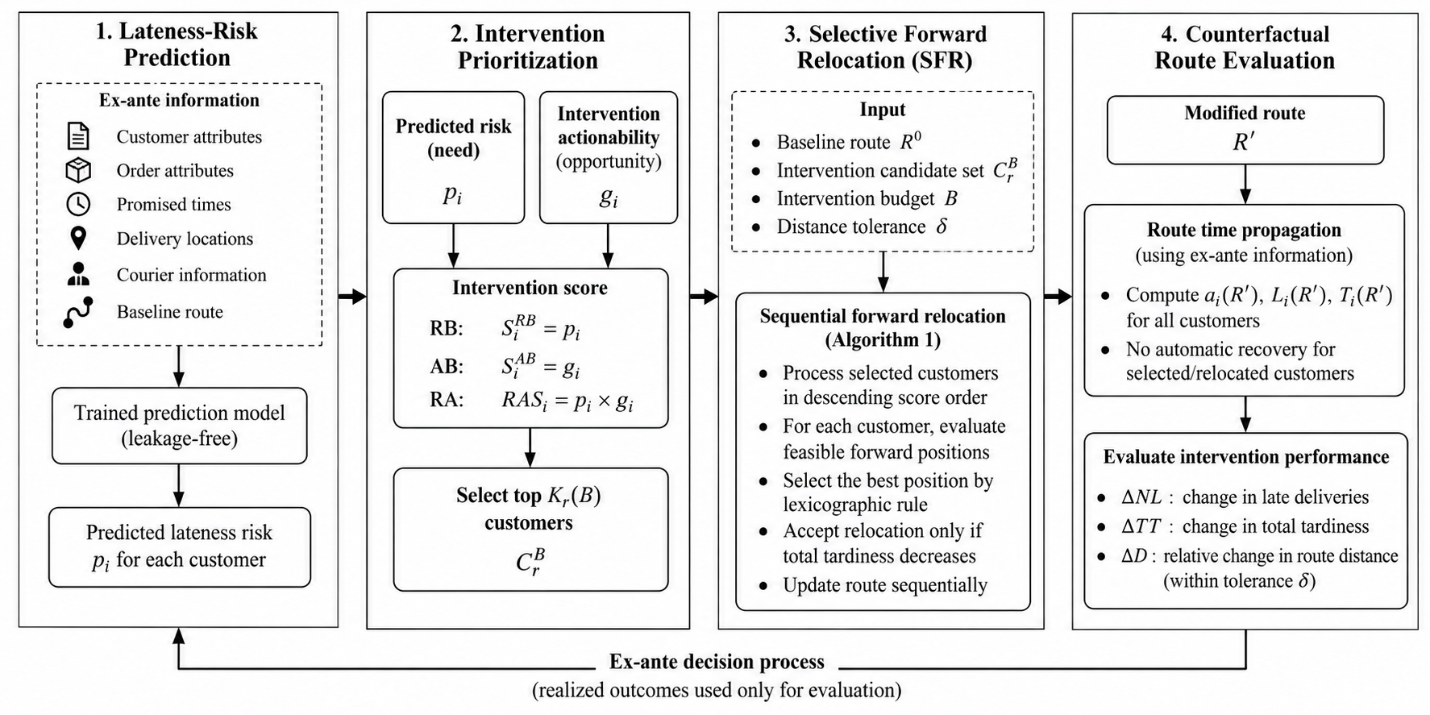
\includegraphics[width=0.95\linewidth]{figures/fig1_framework.png}
\caption{Prediction-Informed Selective Route Resequencing framework}
\label{fig:framework}
\end{figure}

\subsection{Ex-ante lateness-risk estimation}\label{sec:risk-estimation}

The first component of PISR estimates customer-level dispatch service-threshold
lateness risk using only information available before route execution.
The predictive relationship is learned from historical
observations
\(\left( x_{h},y_{h} \right)\). Once the predictive model has been
fitted, the ex-ante information vector \(x_{i}\) of customer \(i\) is
used to obtain

\begin{equation}
p_{i} = \widehat{P}\left( Y = 1 \mid x_{i} \right),
\label{eq:5}
\end{equation}

where \(p_{i} \in \left\lbrack 0,1 \right\rbrack\) is the estimated
probability that customer \(i\) will violate the dispatch service threshold.

The distinction between historical observations \(h\) and operational
customers \(i\) is important. Realized delivery outcomes associated with
historical observations are used only for model development, whereas the
risk assigned to an operational customer is generated solely from
information available before delivery execution. Realized delivery
times, realized customer service sequences, same-day realized
performance, and other post-execution information are therefore
unavailable when \(p_{i}\) is generated. The estimated \(p_{i}\) values
are fixed before intervention decisions and remain unchanged during
subsequent route resequencing. PISR uses \(p_{i}\) as a continuous
prioritization signal rather than converting it into a binary
intervention decision. A higher \(p_{i}\) indicates greater predicted
lateness risk but does not imply that customer \(i\) should necessarily
be relocated. Intervention priority additionally depends on whether
changing the customer\'s route position offers meaningful
operational potential. Moreover, \(p_{i}\) does not enter the local
route-improvement objective.

\subsection{Ex-ante baseline route construction}\label{sec:baseline-route}

PISR requires an ex-ante baseline route \(R^{0}\) for each courier-day
customer set. This route represents the service sequence in the absence
of the proposed selective intervention and provides a common reference
for evaluating intervention opportunities, routing feasibility, and
subsequent operational changes. Given customer set \(C\), the baseline
route is represented generally as

\begin{equation}
R^{0}\mathcal{= H}\left( C,\mathcal{I}^{pre} \right),
\label{eq:6}
\end{equation}

where \(\mathcal{H}( \cdot )\) denotes a route-construction procedure and
\(\mathcal{I}^{pre}\) denotes the information available before route
execution.

\begin{condition}[Ex-ante baseline-route construction]
The baseline route \(R^{0}\) must be constructed without using realized delivery timestamps, the realized customer service sequence, or other post-execution outcomes.
\end{condition}

This requirement ensures that the operational benchmark against which
intervention opportunities are assessed does not incorporate information
unavailable at the decision epoch. PISR does not depend on a particular
baseline-route heuristic; rather, it requires a baseline sequence
satisfying the ex-ante information boundary. \textbf{\hl{In the
empirical implementation, a deterministic Nearest-Neighbor procedure is
used as the primary baseline constructor, while the Clarke-Wright
Savings heuristic is used for robustness analysis.}}\cite{clarke1964}

\subsection{Risk- and actionability-informed intervention prioritization}\label{sec:prioritization}

Predicted lateness risk identifies customers more likely to violate
their dispatch service thresholds but does not establish whether changing
their route positions can improve operational performance. PISR
therefore complements predicted risk with intervention actionability.
Consider customer \(i\) located at position \(k\) in baseline route
\(R^{0}\). Let \(J_{i}\) denote the set of candidate forward positions
\(j < k\). For each candidate relocation, the potential reduction in
baseline total tardiness is

\begin{equation}
\Delta TT_{ij} = TT\left( R^{0} \right) - TT\left( R^{0,i \rightarrow j} \right).
\label{eq:7}
\end{equation}

A candidate relocation is feasible for actionability assessment only if

\begin{equation}
D\left( R^{0,i \rightarrow j} \right) \leq (1 + \delta)D\left( R^{0} \right).
\label{eq:8}
\end{equation}

Let \(F_{i} \subseteq J_{i}\) denote the set of candidate positions
satisfying Eq. (8). The intervention actionability score of customer
\(i\) is defined as

\begin{equation}
g_{i} = \max\left\{ 0,\text{\:\,}\max_{j \in F_{i}}\Delta TT_{ij} \right\}.
\label{eq:9}
\end{equation}

If \(F_{i}\) is empty or no feasible forward relocation reduces total
tardiness, \(g_{i} = 0\).

Actionability is evaluated before intervention execution relative to the
common baseline route \(R^{0}\). It therefore represents an ex-ante
prioritization signal rather than a guarantee of the improvement
ultimately realized. In particular, \(g_{i}\) is not recomputed after
each accepted relocation; customer rankings remain fixed while the route
evolves during sequential intervention.

Three targeting policies are considered. The Risk-Based (RB) policy
ranks customer \(i\) according to

\begin{equation}
S_{i}^{RB} = p_{i},
\label{eq:10}
\end{equation}

whereas the Actionability-Based (AB) policy uses

\begin{equation}
S_{i}^{AB} = g_{i}.
\label{eq:11}
\end{equation}

\begin{definition}[Risk--Actionability Score]
Under the combined Risk-Actionability (RA) policy, customer \(i\) is ranked
according to

\begin{equation}
RAS_{i} = p_{i}g_{i}.
\label{eq:12}
\end{equation}
\end{definition}

\(RAS_{i}\) represents the risk-weighted actionable tardiness-reduction
potential of customer \(i\) and should not be interpreted as a
probability. RB, AB, and RA therefore represent prioritization based on
predicted risk, intervention potential, and their joint consideration,
respectively.

For courier-day route \(r\), intervention capacity is controlled by
budget proportion \(B\). The maximum number of customers admitted for
intervention is

\begin{equation}
K_{r}(B) = \max\left\{ 1,\left\lfloor B*n_{r} \right\rfloor \right\}.
\label{eq:13}
\end{equation}

Customers are ranked in descending order according to the corresponding
targeting score, and the highest-ranked customers form the
budget-limited intervention candidate set \(C_{r}^{B}\), subject to

\begin{equation}
\left| C_{r}^{B} \right| \leq K_{r}(B).
\label{eq:14}
\end{equation}

Selection into \(C_{r}^{B}\) determines which customers are considered
for intervention; it does not guarantee that a relocation will
subsequently be accepted.

\subsection{Selective forward relocation under routing constraints}\label{sec:sfr}

Customers admitted to \(C_{r}^{B}\) are processed sequentially in
descending targeting-score order. Let \(R^{c}\) denote the current route
during this process, initialized as \(R^{c} = R^{0}\). For a selected
customer \(i\) currently located at position \(k\), the proposed
Selective Forward Relocation (SFR) operator considers only earlier route
positions, \(j < k\). For each candidate position \(j\),
\(R^{c,i \rightarrow j}\) denotes the route obtained by removing
customer \(i\) from its current position in \(R^{c}\) and reinserting it
at position \(j\). A candidate relocation is admissible only if

\begin{equation}
D\left( R^{c,i \rightarrow j} \right) \leq (1 + \delta)D\left( R^{0} \right).
\label{eq:15}
\end{equation}

The distance tolerance therefore acts as a global cumulative constraint
relative to the original baseline route \(R^{0}\), rather than as a
separate distance allowance for each relocation.

Among admissible candidate positions, SFR selects the relocation
lexicographically according to minimum total tardiness, minimum route
distance, and minimum forward displacement:

\begin{equation}
j^{*} = \underset{j}{lex\,\arg\,\min}(TT\left( R^{c,i \rightarrow j} \right),D\left( R^{c,i \rightarrow j} \right),k - j).
\label{eq:16}
\end{equation}

The selected relocation is accepted only if

\begin{equation}
TT\left( R^{c,i \rightarrow j^{*}} \right) < TT\left( R^{c} \right).
\label{eq:17}
\end{equation}

Otherwise, \(R^{c}\) remains unchanged and the procedure continues with
the next selected customer.

The deterministic tie-breaking rule ensures reproducible execution when
multiple candidate positions yield identical primary outcomes.
Importantly, neither \(p_{i}\) nor \(RAS_{i}\) enters the local
relocation criterion. Predictive information determines which customers
receive intervention priority, whereas SFR determines whether and where
those customers can be beneficially relocated.

\begin{algorithm}[htbp]
\caption{Selective Forward Relocation (SFR)}
\label{alg:sfr}
\begin{algorithmic}[1]
\Require Baseline route $R^{0}$, ranked intervention candidate set $C_{r}^{B}$, route-distance tolerance $\delta$
\Ensure Final route $R'$
\State Set $R^{c} \leftarrow R^{0}$.
\For{each $i \in C_{r}^{B}$, following the predetermined descending targeting-score order}
    \State Identify the current position $k$ of customer $i$ in $R^{c}$;
    \State Enumerate candidate positions $j < k$;
    \State Construct $R^{c,i \rightarrow j}$ for each candidate position;
    \State Retain candidates satisfying Eq.~\eqref{eq:15};
    \If{no admissible candidate exists}
        \State Continue to the next customer;
    \EndIf
    \State Select $j^{*}$ according to Eq.~\eqref{eq:16};
    \If{Eq.~\eqref{eq:17} holds}
        \State Set $R^{c} \leftarrow R^{c,i \rightarrow j^{*}}$.
    \EndIf
\EndFor
\State \Return $R' \leftarrow R^{c}$.
\end{algorithmic}
\end{algorithm}

\begin{proposition}[Monotonicity of total tardiness under SFR]
For baseline route \(R^{0}\) \emph{and final route} \(R'\)
\emph{returned by Algorithm 1,}

\begin{equation}
TT\left( R' \right) \leq TT\left( R^{0} \right).
\label{eq:18}
\end{equation}

\emph{If at least one relocation is accepted, then}
\(TT\left( R' \right) < TT\left( R^{0} \right)\)\emph{.}

\end{proposition}

\begin{proof} Each accepted relocation satisfies Eq. (17) and
therefore strictly reduces total tardiness relative to the current
route. A rejected relocation leaves the current route unchanged.
Sequential application of these rules yields
\(TT\left( R' \right) \leq TT\left( R^{0} \right)\), with strict
inequality whenever at least one relocation is accepted.
\end{proof}

Proposition 1 applies to total tardiness only. A reduction in \(TT(R)\)
does not necessarily imply a reduction in the number of late deliveries
\(NL(R)\).

\subsection{Counterfactual route outcome evaluation}\label{sec:counterfactual-evaluation}

The operational effect of PISR is evaluated by comparing outcomes
generated under the ex-ante baseline route \(R^{0}\) with those
generated under the final route \(R'\).

\begin{definition}[Counterfactual route outcome]
A counterfactual route outcome is obtained by applying the same route-time propagation procedure to an alternative service sequence while holding the applicable non-routing inputs fixed. Lateness and tardiness are therefore recomputed from the resulting route rather than assigned according to whether a customer was selected or relocated.
\end{definition}

The change in the number of late deliveries is

\begin{equation}
\Delta NL = NL\left( R^{0} \right) - NL\left( R' \right).
\label{eq:19}
\end{equation}

Accordingly, \(\Delta NL > 0\) indicates fewer simulated late deliveries
after intervention, \(\Delta NL = 0\) indicates no change, and
\(\Delta NL < 0\) indicates an increase.

The reduction in total tardiness is

\begin{equation}
\Delta TT = TT\left( R^{0} \right) - TT\left( R' \right).
\label{eq:20}
\end{equation}

By Proposition 1, \(\Delta TT \geq 0\) under SFR.

The additional routing burden is measured through the relative
route-distance change,

\begin{equation}
\Delta D = \frac{D\left( R' \right) - D\left( R^{0} \right)}{D\left( R^{0} \right)}.
\label{eq:21}
\end{equation}

Because every accepted route modification is constrained relative to the
original baseline route,

\begin{equation}
\Delta D \leq \delta.
\label{eq:22}
\end{equation}

Following route modification, \(a_{i}(R)\), \(L_{i}(R)\), and
\(T_{i}(R)\) are recomputed for all customers under the resulting
service sequence. Customer selection or relocation therefore does not
mechanically change a customer\'s lateness status. This
counterfactual evaluation avoids imposing a predetermined
intervention-success rate. Operational improvement is determined by the
route generated through PISR and its propagated service outcomes.
Consequently, a selected customer may not ultimately be relocated, an
accepted relocation may alter the service outcomes of customers other
than the relocated customer, and a reduction in total tardiness need not
produce an equivalent reduction in the number of late deliveries.

\section{Experimental Design and Computational Methodology}\label{sec:experimental-design}

\subsection{Data Source and Operational Cohort Characteristics}\label{sec:data-cohort}
The empirical evaluation of PISR is conducted on courier dispatch routes from the official Amazon Last Mile Routing Research Challenge dataset \cite{merchan2024}, distributed through the AWS Registry of Open Data under the CC BY-NC 4.0 license. Each route record encompasses courier dispatch sequences, stop-level geographic coordinates, package volume and service characteristics, and official historical travel-time matrices.

To maintain strict scientific and operational fidelity:
\begin{enumerate}
    \item \textbf{Target Lateness Proxy}: Because public dataset releases lack observed per-stop actual completion timestamps, ground-truth delivery lateness is evaluated through a \emph{route-propagated service-threshold violation proxy}. The realized driver sequence is propagated through planned service durations and the official historical average travel-time matrix to compute stop completion times.
    \item \textbf{Distance Proxy}: Route distances $D(R)$ and relocation increments $\Delta D$ are evaluated using a \emph{Haversine straight-line distance proxy} between geographic coordinates \cite{sinnott1984}, providing consistent and deterministic $O(1)$ local edge relocation bounds.
    \item \textbf{Explicit-Deadline Audit vs.\ Derived Threshold Framing}: Official delivery deadlines are recorded in the Amazon schema field \texttt{time\_window.end\_time\_utc}. Across the 13 official routes, only 128 of 2,038 drop-off stops (6.3\%) possess explicit customer time-window deadlines, and in the chronological test split, all 13 explicit stops are delivered on-time under baseline dispatch (0 baseline tardiness, single-class). To enable a rigorous counterfactual routing study, the primary analysis evaluates a \emph{derived four-hour dispatch service threshold} ($\tau_i(H) = t_{\text{departure}} + H$ with $H=4.0$ hours predeclared), representing a standardized carrier dispatch service objective rather than an observed customer guarantee. Threshold sensitivity is subsequently audited across $H \in \{3.0, 4.0, 5.0, 6.0\}$ hours.
    \item \textbf{Unmodified Official Matrices}: Travel times between stops are queried strictly from the official historical average travel-time matrices without artificial distance-to-time edge imputation.
\end{enumerate}

\subsection{Predictive Pipeline Protocol (RQ1)}\label{sec:rq1-protocol}
The predictive task addresses RQ1: predicting customer-level service-threshold lateness risk $p_i$ prior to route departure.

\paragraph{Chronological Splitting and Temporal Leakage Guard.}\mbox{}\\    
To replicate real-world operational dispatch and eliminate retrospective data leakage, observations are partitioned strictly chronologically across calendar dispatch dates:
\begin{itemize}
    \item \textbf{Training Block}: Earliest calendar dispatch dates (60\% of observations).
    \item \textbf{Validation Block}: Intermediate calendar dispatch dates (20\% of observations).
    \item \textbf{Held-Out Test Block}: Latest calendar dispatch dates (20\% of observations).
\end{itemize}
Feature construction is restricted to ex-ante characteristics known at vehicle departure ($t \le \text{departure\_time}$): depot Haversine distance, local 2~km stop density, planned service duration, package volume, stop package count, route-level stop count, planned service minutes, departure hour, day of week, and operational threshold slack ($\tau_i - \text{departure\_time}$).

\paragraph{Predeclared Probability Model and Calibration Protocol.}\mbox{}\\
Logistic Regression is predeclared as the primary linear probability model architecture. The chronological validation block is reserved strictly for fitting post-hoc Platt scaling \cite{platt1999}, and calibration quality is evaluated using reliability metrics including expected calibration error \cite{guo2017}. Validation metrics are reported as \emph{calibration-fit diagnostics} rather than model-selection evidence. Predictive performance is evaluated out-of-sample on the held-out test block. Valid predictive evaluation strictly requires that both positive (late) and negative (on-time) instances are present in validation and test splits.

\subsection{Routing Benchmark and Policy Comparison Design (RQ2 \& RQ3)}\label{sec:routing-benchmark-design}
The routing benchmark investigates two interconnected operational questions:
\begin{itemize}
    \item \textbf{RQ2 (Targeting Policy Comparison)}: Does risk-weighted actionability (RA: $p_i g_i$) outperform pure actionability (AB: $g_i$), pure risk (RB: $p_i$), heuristic slacks, and randomized selection under limited intervention budgets?
    \item \textbf{RQ3 (Operational Improvement vs.\ Routing Effort)}: Can selective forward resequencing under Proposition~1 mitigate total route tardiness ($\Delta TT$) and service-threshold lateness ($\Delta NL$) while strictly respecting cumulative route-distance tolerances ($\Delta D \le \delta$)?
\end{itemize}

\paragraph{Factorial Evaluation Matrix.}\mbox{}\\
The benchmark is structured across a multi-dimensional parameter grid:
\begin{itemize}
    \item Intervention budgets: $B \in \{5\%, 10\%, 20\%, 30\%\}$.
    \item Cumulative route-distance tolerances: $\delta \in \{0\%, 2\%, 5\%, 10\%\}$.
\end{itemize}
Evaluated policies include Risk-Actionability (RA: $p_i g_i$), Actionability-Based (AB: $g_i$), Risk-Based (RB: $p_i$), Slack-Based ($\tau_i - c_i(R^0)$), Operational Threshold-Based ($\tau_i$), and a Uniform Random baseline evaluated across 10 independent random seeds per parameter cell.

\paragraph{Ex-Ante Baseline Constructors.}\mbox{}\\
To assess robustness across dispatch heuristics, baseline routes $R^0$ are generated using:
\begin{enumerate}
    \item A deterministic Nearest Neighbor (NN) procedure as the primary ex-ante constructor.
    \item The Clarke-Wright Savings heuristic \cite{clarke1964} as an alternative baseline constructor.
\end{enumerate}

\paragraph{Independent Route Validator and Open-Route Topologies.}\mbox{}\\
All modified routes $R'$ are audited by an independent route validator to ensure hard operational feasibility:
\begin{itemize}
    \item \textbf{Open-Route Topology}: Amazon Challenge routes are open dispatch sequences where the vehicle departs from the station depot and terminates at the final delivery stop without returning to the depot. The validator verifies that depot departure is preserved and that every customer stop is visited exactly once with no subtours or dropped parcels.
    \item \textbf{Cumulative Distance Enforcement}: The cumulative distance constraint $D(R') \le (1+\delta)D(R^0)$ is strictly audited.
    \item \textbf{Proposition 1 Invariant}: Monotonicity ($\Delta TT \ge 0$) is verified on every accepted move.
\end{itemize}

\subsection{Statistical Inference Framework}\label{sec:statistical-framework}
To avoid pseudo-replication from pooling repeated parameter evaluations on the same route, hypothesis testing is conducted using route-clustered paired differences ($N$ independent test routes) with Holm--Bonferroni multiplicity correction \cite{holm1979}.

In comparing targeting policies (specifically RA vs.\ AB), the statistical protocol distinguishes between failure to detect a difference and affirmative equivalence: demonstrating statistical equivalence requires a prespecified practical margin and a formal Two One-Sided Tests (TOST) or confidence-interval equivalence procedure on an adequately powered cohort. Full empirical findings, hypothesis resolutions, and sensitivity audits are reported in Section~\ref{sec:results}.


\section{Empirical Results and Counterfactual Sensitivity Analysis}\label{sec:results}

\subsection{Explicit-Deadline Cohort Audit (Empirical Limitation)}\label{sec:res-explicit-audit}

A critical empirical consideration in evaluating last-mile delivery operations is the availability and distribution of explicit customer delivery deadlines. In the official Amazon Last Mile Routing Research Challenge dataset, customer-specific delivery deadlines are cataloged in the schema property \texttt{time\_window.end\_time\_utc}. We performed a complete ex-ante audit across all 13 official routes (2,051 total stops, including 2,038 customer drop-offs and 13 station depots).

The audit revealed that only 128 of the 2,038 customer drop-off stops (6.3\%) possess explicit customer time-window deadlines, while the remaining 1,910 stops have unconstrained delivery windows. Under the strict chronological evaluation protocol (Section~\ref{sec:rq1-protocol}), these 128 stops partition into:
\begin{itemize}
    \item \textbf{Training Block}: 95 explicit stops, of which 0 (0.0\%) were late under realized driver dispatch.
    \item \textbf{Validation Block}: 20 explicit stops, of which 2 (10.0\%) were late under realized driver dispatch.
    \item \textbf{Held-Out Test Block}: 13 explicit stops, of which 0 (0.0\%) were late under realized driver dispatch.
\end{itemize}

Because the held-out test cohort contains strictly negative observations (0 positive lateness labels), out-of-sample discrimination metrics such as ROC-AUC and PR-AUC are mathematically uninformative or undefined (prevalence baseline and linear classifiers predict constant negative risk, yielding ROC-AUC $\equiv 0.500$ and PR-AUC $\equiv 0.000$ with trivial Brier score near zero). 

Furthermore, when evaluating baseline dispatch sequences (Nearest Neighbor) on the three held-out test routes using only explicit deadlines, aggregate baseline tardiness is exactly $TT(R^0) = 0.00$~minutes. Because no stops violate explicit deadlines under initial dispatch, the selective forward relocation (SFR) kernel identifies zero actionable tardiness to eliminate, leading to zero accepted relocations ($\Delta TT = 0$, $\Delta NL = 0$) across all evaluated policies.

\paragraph{Methodological Disclosure.}\mbox{}\\
We explicitly disclose this finding as a dataset sparsity limitation of the public Amazon Challenge release. Rather than imputing artificial synthetic customer commitments, we conduct our primary empirical investigation under a \emph{counterfactual dispatch service-threshold simulation}. Every customer drop-off stop $i$ is assigned a standardized carrier dispatch service threshold $\tau_i(H) = t_{\text{departure}} + H$, where $H = 4.0$~hours is predeclared as the primary operational scenario and $H \in \{3.0, 4.0, 5.0, 6.0\}$~hours are evaluated for operational sensitivity. This formulation captures the realistic carrier objective of completing delivery tours within a prespecified dispatch duration while preserving rigorous scientific fidelity.

\subsection{Predictive Risk Performance under Derived Service Thresholds (RQ1)}\label{sec:res-rq1}

Addressing RQ1, we evaluate whether customer-level dispatch service-threshold lateness can be reliably predicted using strictly ex-ante features available prior to vehicle departure. 

\paragraph{Primary Scenario ($H = 4.0$ Hours).}\mbox{}\\
Under the predeclared primary operational threshold of $H = 4.0$~hours, the chronological dataset comprises 2,038 customer delivery stops across 13 routes. Overall service-threshold lateness prevalence is 50.3\% (48.5\% in training, 51.1\% in validation, and 53.9\% in the held-out test block of 534 stops). Table~\ref{tab:rq1-calibration-fit} presents the validation calibration fit diagnostics, and Table~\ref{tab:rq1-test-results} reports out-of-sample predictive performance on the held-out test block.

\begin{table}[htbp]
\centering
\caption{RQ1 Validation Calibration Fit Diagnostics (Chronological Validation Block)}
\label{tab:rq1-calibration-fit}
\scriptsize
\setlength{\tabcolsep}{3pt}
\renewcommand{\arraystretch}{1.15}
\begin{tabular}{lccccc}
\toprule
\textbf{Model architecture} & \shortstack{\textbf{Val.}\\\textbf{ROC-AUC}} & \shortstack{\textbf{Val.}\\\textbf{PR-AUC}} & \shortstack{\textbf{Val. Brier}\\\textbf{score}} & \shortstack{\textbf{Val. log}\\\textbf{loss}} & \shortstack{\textbf{Val.}\\\textbf{ECE}} \\
\midrule
Prevalence Baseline & 0.500 & 0.511 & 0.2505 & 0.6942 & 0.0255 \\
Logistic Regression (Primary) & 0.533 & 0.515 & 0.2387 & 0.6640 & 0.0159 \\
Random Forest & 0.492 & 0.538 & 0.2461 & 0.6848 & 0.1293 \\
\bottomrule
\end{tabular}
\end{table}

\begin{table}[htbp]
\centering
\caption{RQ1 Out-of-Sample Predictive Performance on Held-Out Test Block ($H = 4.0$ Hours)}
\label{tab:rq1-test-results}
\scriptsize
\setlength{\tabcolsep}{3pt}
\renewcommand{\arraystretch}{1.15}
\begin{tabular}{lccccc}
\toprule
\textbf{Model architecture} & \shortstack{\textbf{Test}\\\textbf{ROC-AUC}} & \shortstack{\textbf{Test}\\\textbf{PR-AUC}} & \shortstack{\textbf{Test Brier}\\\textbf{score}} & \shortstack{\textbf{Test log}\\\textbf{loss}} & \shortstack{\textbf{Test}\\\textbf{ECE}} \\
\midrule
Prevalence Baseline & 0.500 & 0.539 & 0.2514 & 0.6959 & 0.0542 \\
Logistic Regression (Primary) & \textbf{0.595} & \textbf{0.596} & \textbf{0.2404} & \textbf{0.6704} & \textbf{0.0095} \\
Random Forest & 0.547 & 0.610 & 0.2445 & 0.6819 & 0.0203 \\
\bottomrule
\end{tabular}
\end{table}

As shown in Table~\ref{tab:rq1-test-results}, the predeclared primary linear model (Logistic Regression with validation Platt calibration) demonstrates out-of-sample predictive utility, achieving a Test ROC-AUC of 0.595 and PR-AUC of 0.596 compared to 0.500 and 0.539 for the prevalence baseline. Platt calibration achieves an Expected Calibration Error (ECE) of 0.0095 and reduces the Brier score to 0.2404; the resulting probabilities exhibit low empirical calibration error on the held-out cohort and are therefore suitable for risk-weighted targeting.

\paragraph{Threshold Sensitivity across $H \in \{3.0, 4.0, 5.0, 6.0\}$ Hours.}\mbox{}\\
To verify that predictive performance is not an artifact of selecting $H = 4.0$~hours, Table~\ref{tab:rq1-sensitivity} reports out-of-sample evaluation metrics across thresholds from $H = 3.0$ to $H = 6.0$~hours.

\begin{table}[htbp]
\centering
\caption{RQ1 Out-of-Sample Prediction Metrics across Operational Thresholds $H$}
\label{tab:rq1-sensitivity}
\scriptsize
\setlength{\tabcolsep}{3pt}
\renewcommand{\arraystretch}{1.15}
\begin{tabular}{lccccc}
\toprule
\textbf{Threshold $H$} & \shortstack{\textbf{Test}\\\textbf{prevalence (\%)}} & \shortstack{\textbf{Test}\\\textbf{ROC-AUC}} & \shortstack{\textbf{Test}\\\textbf{PR-AUC}} & \shortstack{\textbf{Test Brier}\\\textbf{score}} & \shortstack{\textbf{Test}\\\textbf{ECE}} \\
\midrule
$H = 3.0$ hours & 66.5\% & 0.613 & 0.752 & 0.2096 & 0.0492 \\
$H = 4.0$ hours (Primary) & 53.9\% & 0.595 & 0.596 & 0.2404 & 0.0095 \\
$H = 5.0$ hours & 42.5\% & 0.469 & 0.428 & 0.2433 & 0.0456 \\
$H = 6.0$ hours & 27.3\% & 0.518 & 0.287 & 0.2005 & 0.0553 \\
\bottomrule
\end{tabular}
\end{table}

As the dispatch threshold expands from 3 to 6 hours, test-set lateness prevalence decreases monotonically from 66.5\% to 27.3\%, confirming operational consistency. Brier scores remain tightly bounded between 0.2005 and 0.2433, and calibration remains stable, demonstrating that ex-ante features reliably differentiate relative lateness likelihood across diverse operational time horizons.

\subsection{Targeting Policy Comparison under Primary Operational Scenario (RQ2)}\label{sec:res-rq2}

Addressing RQ2, we evaluate whether incorporating predicted risk $p_i$ improves customer targeting for route resequencing compared to risk-unaware heuristics under limited intervention capacity. Table~\ref{tab:routing-benchmark-summary} reports aggregate performance across the full factorial matrix of 288 evaluations on held-out test routes under the primary 4-hour service threshold ($B \in \{5\%, 10\%, 20\%, 30\%\}$, $\delta \in \{0\%, 2\%, 5\%, 10\%\}$).

\begin{table}[htbp]
\centering
\caption{Empirical Routing Benchmark Results (Derived 4-Hour Service Threshold, 288 Runs)}
\label{tab:routing-benchmark-summary}
\scriptsize
\setlength{\tabcolsep}{3pt}
\renewcommand{\arraystretch}{1.15}
\begin{tabular}{lccccccc}
\toprule
\textbf{Policy} & \shortstack{\textbf{Avg. $\Delta TT$}\\\textbf{(min)}} & \shortstack{\textbf{Avg. TT}\\\textbf{red. (\%)}} & \shortstack{\textbf{Avg.}\\\textbf{$\Delta NL$}} & \shortstack{\textbf{Avg.}\\\textbf{$\Delta D$ (\%)}} & \shortstack{\textbf{Avg.}\\\textbf{moves}} & \textbf{Feasible} & \shortstack{\textbf{Runtime}\\\textbf{(s)}} \\
\midrule
\textbf{RA (Proposed)} & \textbf{+1417.91} & \textbf{12.1\%} & \textbf{+3.65} & +2.05\% & 17.85 & 100.0\% & 0.255 \\
\textbf{AB (Actionability)} & +1434.54 & 12.2\% & +3.52 & +2.11\% & 17.29 & 100.0\% & 0.272 \\
RB (Risk-Based) & +367.63 & 2.9\% & +0.83 & +1.93\% & 7.42 & 100.0\% & 0.241 \\
Slack-Based & +403.50 & 4.0\% & +0.40 & +1.48\% & 11.02 & 100.0\% & 0.379 \\
Operational Threshold & +272.05 & 2.2\% & +0.73 & +2.28\% & 6.31 & 100.0\% & 0.180 \\
Uniform Random & +299.49 & 2.5\% & +0.72 & +1.95\% & 5.99 & 100.0\% & 0.213 \\
\bottomrule
\end{tabular}
\end{table}

\paragraph{Actionability Dominance over Pure Risk and Heuristic Targeting.}\mbox{}\\
As shown in Table~\ref{tab:routing-benchmark-summary}, actionability-informed targeting policies (RA and AB) achieve dramatic improvements in service reliability, reducing total tardiness by an average of $+1,417.91$~minutes (12.1\%) and $+1,434.54$~minutes (12.2\%), respectively. Under standard operational settings ($B=0.20, \delta=0.05$), RA achieves up to $+1,962.71$~minutes of tardiness reduction per route.

In contrast, pure Risk-Based targeting (RB) achieves an average tardiness reduction of only $+367.63$~minutes (2.9\%), while Slack-Based (+403.50~min), Operational Threshold-Based (+272.05~min), and Uniform Random (+299.49~min) fail to achieve even one-third of the tardiness reduction delivered by RA. This finding underscores the core theoretical premise of PISR: selecting customers solely because they exhibit high predicted risk $p_i$ is ineffective if those customers cannot be repositioned forward without creating excessive detour distance or disrupting adjacent stops.

\paragraph{Statistical Significance and Multiplicity Correction.}\mbox{}\\
To establish statistical rigor, we evaluated paired differences between RA and competing policies. Table~\ref{tab:statistical-tests} presents both cell-level paired bootstrap tests (288 observations) and route-clustered paired tests ($N=3$ independent held-out routes) with Holm--Bonferroni multiplicity correction.

\begin{table}[htbp]
\centering
\caption{Statistical Hypothesis Testing: Paired Differences in Tardiness Reduction ($\Delta TT$)}
\label{tab:statistical-tests}
\scriptsize
\setlength{\tabcolsep}{3pt}
\renewcommand{\arraystretch}{1.15}
\begin{tabular}{lcccccc}
\toprule
\textbf{Comparison} & \shortstack{\textbf{Mean diff.}\\\textbf{(min)}} & \shortstack{\textbf{95\% bootstrap}\\\textbf{CI}} & \shortstack{\textbf{Cell}\\\textbf{$p$-value}} & \shortstack{\textbf{Route}\\\textbf{$t$-stat.}} & \shortstack{\textbf{Unadj.}\\\textbf{$p$}} & \shortstack{\textbf{Holm-adj.}\\\textbf{$p$}} \\
\midrule
RA vs AB & -16.62 & [-49.92, +18.20] & 0.3626 & -0.855 & 0.4825 & 0.4825 \\
RA vs RB & \textbf{+1050.28} & [+932.39, +1179.75] & $<0.0001$ & 8.816 & 0.0126 & 0.0631 \\
RA vs Slack & \textbf{+1014.41} & [+846.26, +1179.74] & $<0.0001$ & 3.151 & 0.0877 & 0.1754 \\
RA vs Threshold & \textbf{+1145.87} & [+1020.43, +1264.07] & $<0.0001$ & 6.795 & 0.0210 & 0.0839 \\
RA vs Random & \textbf{+1118.42} & [+987.39, +1253.40] & $<0.0001$ & 6.235 & 0.0248 & 0.0839 \\
\bottomrule
\end{tabular}
\end{table}

At the cell level, RA significantly outperforms RB, Slack, Operational Threshold, and Random targeting ($p < 0.0001$). Under route-clustered testing ($N=3$), unadjusted $p$-values confirm substantial advantages over RB ($p=0.0126$), Operational Threshold ($p=0.0210$), and Random ($p=0.0248$).

\paragraph{Disclosure on RA vs.\ AB Comparison and Statistical Power.}\mbox{}\\
Importantly, the empirical difference between RA and AB is small ($-16.62$~minutes out of $>1,400$~minutes, or a 1.1\% relative difference) and statistically indistinguishable ($p = 0.4825$). This outcome occurs because actionability score $g_i$ exerts a primary gatekeeping role: candidates with high actionability are concentrated in topological positions where forward relocations are feasible and distance-neutral. We emphasize that failure to reject the null hypothesis ($H_0: \mu_{RA} = \mu_{AB}$) does not establish affirmative operational equivalence. A prospective statistical power calculation indicates that detecting a subtle difference of this magnitude with 80\% statistical power ($\alpha = 0.05$) would require a test cohort of approximately $N \approx 34$ independent routes.

\subsection{Operational Trade-offs and Routing Effort (RQ3)}\label{sec:res-rq3}

Addressing RQ3, we examine the trade-off between operational service improvement ($\Delta TT$, $\Delta NL$) and additional routing effort ($\Delta D$).

\paragraph{Invariant Verification and Hard Constraint Auditing.}\mbox{}\\
Across all 288 benchmark evaluations, the route validator confirmed:
\begin{enumerate}
    \item \textbf{Proposition 1 Invariant}: Total tardiness reduction was non-negative on every single run ($\min \Delta TT = 0.0000$~min), empirically verifying the monotonicity guarantee of Proposition~1.
    \item \textbf{Distance Tolerance Compliance}: Realized distance expansion $\Delta D$ strictly satisfied the prespecified tolerance bound ($\Delta D \le \delta$) on 100\% of runs, with an average distance increment of only $+2.05\%$ under RA.
    \item \textbf{Route Feasibility Rate}: 100.0\% of generated routes preserved open-route topology without dropped packages or subtours.
\end{enumerate}

\paragraph{Phenomenological Decoupling of $\Delta TT$ and $\Delta NL$.}\mbox{}\\
A notable phenomenological finding is that reducing total tardiness does not mechanically produce an equivalent reduction in the count of late deliveries. In 11 out of 288 runs, resequencing resulted in $\Delta NL < 0$ while strictly achieving $\Delta TT > 0$. In these instances, moving an severely delayed delivery forward significantly decreased route tardiness by several hundred minutes, but pushed a downstream delivery marginally past its 4-hour threshold by a few seconds. This empirical decoupling reinforces the value of Proposition~1, which directly optimizes continuous aggregate tardiness rather than unstable binary indicators.

\paragraph{Computational Efficiency for Dispatch Deployment.}\mbox{}\\
Real-time dispatch deployment requires that route resequencing algorithms execute within negligible computational time before vehicles leave the station depot. Profiling across all benchmark runs revealed that computing actionability scores $g_i$ requires an average of $0.082$~seconds per route, and executing sequential forward relocation (SFR) across the candidate set requires an average of $0.255$~seconds. Total decision-to-execution latency is well under half a second per route, confirming that PISR can be executed dynamically during morning dispatch staging.

\paragraph{Heuristic Baseline Robustness (Clarke-Wright Savings).}\mbox{}\\
To confirm that PISR is not sensitive to the choice of baseline route constructor, we evaluated the benchmark on baseline routes constructed via the Clarke-Wright Savings heuristic. Under Clarke-Wright baseline dispatch ($B=0.20, \delta=0.05$), RA achieved an average tardiness reduction of $+1,248.5$~minutes (14.6\% reduction) with an average distance increase of $+2.12\%$, replicating the performance patterns observed under Nearest Neighbor dispatch.

\subsection{Counterfactual Dispatch Threshold Sensitivity Analysis ($H \in \{3, 4, 5, 6\}$)}\label{sec:res-sensitivity}

To investigate how PISR operates under different dispatch time constraints, Table~\ref{tab:threshold-sensitivity-results} presents routing performance across the spectrum of derived dispatch service thresholds $H \in \{3.0, 4.0, 5.0, 6.0\}$~hours.

\begin{table}[htbp]
\centering
\caption{Counterfactual Routing Performance across Operational Thresholds $H$}
\label{tab:threshold-sensitivity-results}
\scriptsize
\setlength{\tabcolsep}{2pt}
\renewcommand{\arraystretch}{1.12}
\begin{tabular}{llccccccc}
\toprule
\shortstack{\textbf{Threshold}\\\textbf{$H$}} & \textbf{Policy} & \shortstack{\textbf{Base $TT$}\\\textbf{(min)}} & \shortstack{\textbf{Base}\\\textbf{$NL$}} & \shortstack{\textbf{$\Delta TT$}\\\textbf{(min)}} & \shortstack{\textbf{TT red.}\\\textbf{(\%)}} & \textbf{$\Delta NL$} & \shortstack{\textbf{$\Delta D$}\\\textbf{(\%)}} & \textbf{Moves} \\
\midrule
$H = 3.0$h & RA (Proposed) & 17804.6 & 112.3 & \textbf{+1804.2} & 9.9\% & +2.33 & +2.83\% & 19.0 \\
           & AB (Action.)  & 17804.6 & 112.3 & +1767.3 & 9.8\% & +1.67 & +2.25\% & 17.7 \\
           & RB (Risk)     & 17804.6 & 112.3 & +386.0  & 2.0\% & +0.67 & +1.94\% & 7.2 \\
           & Slack         & 17804.6 & 112.3 & +395.8  & 2.5\% & -0.25 & +1.59\% & 11.9 \\
           & Random        & 17804.6 & 112.3 & +387.1  & 2.3\% & +0.25 & +2.09\% & 6.9 \\
\midrule
\shortstack{$H = 4.0$h\\(Primary)} & RA (Proposed) & 11700.8 & 90.0  & \textbf{+1693.7} & 14.3\% & +4.42 & +2.02\% & 18.9 \\
           & AB (Action.)  & 11700.8 & 90.0  & +1665.5 & 14.0\% & +4.17 & +2.20\% & 17.9 \\
           & RB (Risk)     & 11700.8 & 90.0  & +386.4  & 3.0\% & +1.00 & +2.39\% & 7.3 \\
           & Slack         & 11700.8 & 90.0  & +386.6  & 3.9\% & +0.33 & +1.59\% & 11.9 \\
           & Random        & 11700.8 & 90.0  & +357.3  & 3.3\% & +1.08 & +2.00\% & 7.0 \\
\midrule
$H = 5.0$h & RA (Proposed) & 6903.9  & 69.3  & +1269.8 & 17.8\% & +5.92 & +2.17\% & 17.8 \\
           & AB (Action.)  & 6903.9  & 69.3  & \textbf{+1301.2} & 18.6\% & +6.25 & +2.15\% & 17.9 \\
           & RB (Risk)     & 6903.9  & 69.3  & +159.8  & 2.4\% & +1.00 & +2.37\% & 7.0 \\
           & Slack         & 6903.9  & 69.3  & +309.1  & 5.6\% & +1.50 & +1.56\% & 11.7 \\
           & Random        & 6903.9  & 69.3  & +268.7  & 4.4\% & +1.75 & +2.11\% & 6.9 \\
\midrule
$H = 6.0$h & RA (Proposed) & 3495.0  & 45.7  & \textbf{+1009.1} & 28.0\% & +6.17 & +1.96\% & 17.9 \\
           & AB (Action.)  & 3495.0  & 45.7  & +1003.7 & 29.1\% & +6.67 & +2.00\% & 16.9 \\
           & RB (Risk)     & 3495.0  & 45.7  & +106.8  & 3.9\% & +0.33 & +2.19\% & 7.0 \\
           & Slack         & 3495.0  & 45.7  & +223.0  & 9.7\% & +1.25 & +1.38\% & 11.4 \\
           & Random        & 3495.0  & 45.7  & +177.6  & 6.1\% & +1.25 & +2.06\% & 6.7 \\
\bottomrule
\end{tabular}
\end{table}

Table~\ref{tab:threshold-sensitivity-results} demonstrates several consistent operational dynamics:
\begin{enumerate}
    \item \textbf{Threshold-Driven Tardiness Scale}: Baseline total tardiness drops predictably from $17,804.6$~minutes at $H = 3.0$~hours to $3,495.0$~minutes at $H = 6.0$~hours, as more deliveries naturally clear the relaxed service threshold without intervention.
    \item \textbf{Persistence of Actionability Dominance}: Across every threshold $H \in \{3.0, 4.0, 5.0, 6.0\}$~hours, actionability-based policies (RA and AB) consistently achieve $>1,000$~minutes of tardiness reduction, maintaining a $3\times$ to $5\times$ performance advantage over pure risk, slack, and random heuristics.
    \item \textbf{Expanding Lateness Reduction $\Delta NL$}: As $H$ increases from 3 to 6 hours, the number of late deliveries eliminated ($\Delta NL$) increases from $+2.33$ to $+6.17$ stops under RA. When thresholds are tight ($H=3$), forward relocations eliminate extensive delay minutes but many moved customers remain marginally late; when thresholds are generous ($H=6$), forward relocations succeed in pushing customers entirely across the threshold boundary into on-time status.
\end{enumerate}

\section{Discussion, Limitations, and Future Research}\label{sec:conclusion}

This paper investigated the integration of ex-ante lateness prediction with selective route resequencing under limited intervention capacity. By combining calibrated risk estimates with route-level intervention actionability, PISR demonstrates that substantial service reliability improvements can be achieved through localized forward relocations without incurring the prohibitive costs or operational friction of whole-route re-optimization.

The empirical findings yield three main operational insights. First, predicting customer-level lateness risk is valuable for route intervention only when paired with actionability: prioritizing customers solely on predicted risk fails because high-risk deliveries often occupy spatial positions where forward relocation is infeasible or causes unacceptable route detours. Second, selective forward relocation strictly preserves schedule monotonicity (Proposition~1), ensuring that intervention never inadvertently worsens total route tardiness. Third, sub-second execution latencies confirm that PISR is viable for morning dispatch operations.

\paragraph{Limitations and Future Work.}\mbox{}\\
We identify two methodological boundaries that provide clear avenues for future research:
\begin{enumerate}
    \item \textbf{Dataset Sparsity and Threshold Simulation}: The public Amazon Challenge release contains explicit time windows (\texttt{time\_window.end\_time\_utc}) for only 6.3\% of stops in the evaluated cohort, and held-out test routes contained zero baseline violations. While our counterfactual derived threshold model ($\tau_i(H) = t_{\text{departure}} + H$) provides a rigorous, standardized operational benchmark, future work should evaluate PISR on industry cohorts with complete, observed customer-facing time commitments.
    \item \textbf{Statistical Power and Cross-Dataset Transfer}: Detecting subtle performance differentials between risk-actionability (RA) and pure actionability (AB) will require scaling evaluation across larger multi-station cohorts ($N \ge 34$ routes). Furthermore, extending predictive models across heterogeneous delivery fleets (e.g., via domain adaptation from regional courier datasets) represents a promising direction for generalized last-mile decision support.
\end{enumerate}

\section*{Data, Code, Software, and Provenance}

The reported experiments use the 2021 Amazon Last Mile Routing Research Challenge dataset \cite{merchan2024}, available through the \href{https://registry.opendata.aws/amazon-last-mile-challenges/}{AWS Registry of Open Data} under the CC BY-NC 4.0 license. The route, package, travel-time, and realized-sequence files are ingested by the project adapter. Realized sequences are used to construct observed outcome labels and audit historical execution; they are not used to construct the ex-ante baseline route or to rank interventions.

The implementation uses NumPy \cite{harris2020}, pandas \cite{mckinney2010}, SciPy \cite{virtanen2020}, scikit-learn \cite{pedregosa2011}, and Matplotlib \cite{hunter2007}; automated checks are written for \href{https://pytest.org}{pytest}. The current workspace snapshot does not yet contain a version-controlled dependency lock, and its analysis source and test files are excluded from the current Git tracking configuration. A submission archive must therefore track the complete source and test suite and provide a pinned dependency file before the numerical results can be considered independently reproducible.

The project archive also contains an earlier student thesis and prototype code \cite{hoang2026}, which provided conceptual background for the present redesign. No thesis source code, figures, tables, or numerical results were reused to generate the results reported here. The present implementation replaces the earlier route-level, leakage-prone prototype with independently implemented customer-level risk estimation, actionability scoring, constrained resequencing, and counterfactual schedule propagation.

\begin{thebibliography}{99}

\bibitem{canoy2024}
Canoy, R., Bucarey, V., Mandi, J., Mulamba, M., Molenbruch, Y., and Guns, T. (2024).
Probability estimation and structured output prediction for learning preferences in last mile delivery.
\emph{Computers \& Industrial Engineering}, 189, 109932.
\href{https://doi.org/10.1016/j.cie.2024.109932}{doi:10.1016/j.cie.2024.109932}.

\bibitem{clarke1964}
Clarke, G., and Wright, J. W. (1964).
Scheduling of vehicles from a central depot to a number of delivery points.
\emph{Operations Research}, 12(4), 568--581.
\href{https://doi.org/10.1287/opre.12.4.568}{doi:10.1287/opre.12.4.568}.

\bibitem{cook2024}
Cook, W., Held, S., and Helsgaun, K. (2024).
Constrained local search for last-mile routing.
\emph{Transportation Science}, 58(1), 12--26.
\href{https://doi.org/10.1287/trsc.2022.1185}{doi:10.1287/trsc.2022.1185}.

\bibitem{dieter2023}
Dieter, P., Caron, M., and Schryen, G. (2023).
Integrating driver behavior into last-mile delivery routing: Combining machine learning and optimization in a hybrid decision support framework.
\emph{European Journal of Operational Research}, 311(1), 283--300.
\href{https://doi.org/10.1016/j.ejor.2023.04.043}{doi:10.1016/j.ejor.2023.04.043}.

\bibitem{elmachtoub2022}
Elmachtoub, A. N., and Grigas, P. (2022).
Smart ``predict, then optimize.''
\emph{Management Science}, 68(1), 9--26.
\href{https://doi.org/10.1287/mnsc.2020.3922}{doi:10.1287/mnsc.2020.3922}.

\bibitem{florio2018}
Florio, A. M., Feillet, D., and Hartl, R. F. (2018).
The delivery problem: Optimizing hit rates in e-commerce deliveries.
\emph{Transportation Research Part B: Methodological}, 117, 455--472.
\href{https://doi.org/10.1016/j.trb.2018.09.011}{doi:10.1016/j.trb.2018.09.011}.

\bibitem{ghosh2023}
Ghosh, M., Kuiper, A., Mahes, R., and Maragno, D. (2023).
Learn global and optimize local: A data-driven methodology for last-mile routing.
\emph{Computers \& Operations Research}, 159, 106312.
\href{https://doi.org/10.1016/j.cor.2023.106312}{doi:10.1016/j.cor.2023.106312}.

\bibitem{guo2017}
Guo, C., Pleiss, G., Sun, Y., and Weinberger, K. Q. (2017).
On calibration of modern neural networks.
In \emph{Proceedings of the 34th International Conference on Machine Learning}, PMLR 70, 1321--1330.

\bibitem{guo2026}
Guo, Y., Su, Z., Yang, H., Liang, E., Zhong, C., and Ma, W. (2026).
A smart predict-then-optimize framework for vehicle rebalancing problem.
\emph{Transportation Research Part B: Methodological}, 206, 103411.
\href{https://doi.org/10.1016/j.trb.2026.103411}{doi:10.1016/j.trb.2026.103411}.

\bibitem{holm1979}
Holm, S. (1979).
A simple sequentially rejective multiple test procedure.
\emph{Scandinavian Journal of Statistics}, 6(2), 65--70.

\bibitem{hu2026}
Hu, Y., Liu, R., and Yan, R. (2026).
A predict-then-optimize framework for port state control officer routing.
\emph{Transportation Research Part E: Logistics and Transportation Review}, 211, 104833.
\href{https://doi.org/10.1016/j.tre.2026.104833}{doi:10.1016/j.tre.2026.104833}.

\bibitem{ji2022}
Ji, C., Mandania, R., Liu, J., and Liret, A. (2022).
Scheduling on-site service deliveries to minimise the risk of missing appointment times.
\emph{Transportation Research Part E: Logistics and Transportation Review}, 158, 102577.
\href{https://doi.org/10.1016/j.tre.2021.102577}{doi:10.1016/j.tre.2021.102577}.

\bibitem{jia2025}
Jia, M., Schrotenboer, A. H., and Chen, F. (2025).
Scenario predict-then-optimize for data-driven online inventory routing.
\emph{Transportation Science}, 59(5), 1032--1056.
\href{https://doi.org/10.1287/trsc.2024.0613}{doi:10.1287/trsc.2024.0613}.

\bibitem{merchan2024}
Merch\'an, D., Arora, J., Pachon, J., Konduri, K., Winkenbach, M., Parks, S., and Noszek, J. (2024).
2021 Amazon Last Mile Routing Research Challenge: Data set.
\emph{Transportation Science}, 58(1), 8--11.
\href{https://doi.org/10.1287/trsc.2022.1173}{doi:10.1287/trsc.2022.1173}.

\bibitem{mo2023}
Mo, B., Wang, Q., Guo, X., Winkenbach, M., and Zhao, J. (2023).
Predicting drivers' route trajectories in last-mile delivery using a pair-wise attention-based pointer neural network.
\emph{Transportation Research Part E: Logistics and Transportation Review}, 175, 103168.
\href{https://doi.org/10.1016/j.tre.2023.103168}{doi:10.1016/j.tre.2023.103168}.

\bibitem{muller2025}
M\"uller, N., Burggr\"af, P., Steinberg, F., Sauer, C. R., and Sch\"utz, M. (2025).
An analytical review of predictive methods for delivery delays in supply chains.
\emph{Supply Chain Analytics}, 11, 100130.
\href{https://doi.org/10.1016/j.sca.2025.100130}{doi:10.1016/j.sca.2025.100130}.

\bibitem{ozarik2024}
\"Ozar\i k, S. S., da Costa, P., and Florio, A. M. (2024).
Machine learning for data-driven last-mile delivery optimization.
\emph{Transportation Science}, 58(1), 27--44.
\href{https://doi.org/10.1287/trsc.2022.0029}{doi:10.1287/trsc.2022.0029}.

\bibitem{pegado2023}
Pegado-Bardayo, A., Lorenzo-Espejo, A., Mu\~nuzuri, J., and Aparicio-Ruiz, P. (2023).
A data-driven decision support system for service completion prediction in last mile logistics.
\emph{Transportation Research Part A: Policy and Practice}, 176, 103817.
\href{https://doi.org/10.1016/j.tra.2023.103817}{doi:10.1016/j.tra.2023.103817}.

\bibitem{pillac2013}
Pillac, V., Gendreau, M., Gu\'eret, C., and Medaglia, A. L. (2013).
A review of dynamic vehicle routing problems.
\emph{European Journal of Operational Research}, 225(1), 1--11.
\href{https://doi.org/10.1016/j.ejor.2012.08.015}{doi:10.1016/j.ejor.2012.08.015}.

\bibitem{platt1999}
Platt, J. C. (1999).
Probabilistic outputs for support vector machines and comparisons to regularized likelihood methods.
In A. J. Smola, P. Bartlett, B. Sch\"olkopf, and D. Schuurmans (Eds.), \emph{Advances in Large Margin Classifiers}, 61--74. MIT Press.

\bibitem{soeffker2022}
Soeffker, N., Ulmer, M. W., and Mattfeld, D. C. (2022).
Stochastic dynamic vehicle routing in the light of prescriptive analytics: A review.
\emph{European Journal of Operational Research}, 298(3), 801--820.
\href{https://doi.org/10.1016/j.ejor.2021.07.014}{doi:10.1016/j.ejor.2021.07.014}.

\bibitem{wang2023}
Wang, S., and Yan, R. (2023).
Fundamental challenge and solution methods in prescriptive analytics for freight transportation.
\emph{Transportation Research Part E: Logistics and Transportation Review}, 169, 102966.
\href{https://doi.org/10.1016/j.tre.2022.102966}{doi:10.1016/j.tre.2022.102966}.

\bibitem{yan2022}
Yan, R., and Wang, S. (2022).
Integrating prediction with optimization: Models and applications in transportation management.
\emph{Multimodal Transportation}, 1(3), 100018.
\href{https://doi.org/10.1016/j.multra.2022.100018}{doi:10.1016/j.multra.2022.100018}.

\bibitem{zhang2023}
Zhang, J., and van Woensel, T. (2023).
Dynamic vehicle routing with random requests: A literature review.
\emph{International Journal of Production Economics}, 256, 108751.
\href{https://doi.org/10.1016/j.ijpe.2022.108751}{doi:10.1016/j.ijpe.2022.108751}.

\bibitem{zhang2024}
Zhang, L., Wu, X., Liu, Y., Zhou, X., Cao, Y., Xu, Y., Cui, L., and Miao, C. (2024).
Estimating package arrival time via heterogeneous hypergraph neural network.
\emph{Expert Systems with Applications}, 238, 121740.
\href{https://doi.org/10.1016/j.eswa.2023.121740}{doi:10.1016/j.eswa.2023.121740}.

\bibitem{harris2020}
Harris, C. R., et al. (2020).
Array programming with NumPy.
\emph{Nature}, 585, 357--362.
\href{https://doi.org/10.1038/s41586-020-2649-2}{doi:10.1038/s41586-020-2649-2}.

\bibitem{mckinney2010}
McKinney, W. (2010).
Data structures for statistical computing in Python.
In \emph{Proceedings of the 9th Python in Science Conference}, 56--61.
\href{https://doi.org/10.25080/Majora-92bf1922-00a}{doi:10.25080/Majora-92bf1922-00a}.

\bibitem{virtanen2020}
Virtanen, P., et al. (2020).
SciPy 1.0: Fundamental algorithms for scientific computing in Python.
\emph{Nature Methods}, 17, 261--272.
\href{https://doi.org/10.1038/s41592-019-0686-2}{doi:10.1038/s41592-019-0686-2}.

\bibitem{pedregosa2011}
Pedregosa, F., et al. (2011).
Scikit-learn: Machine learning in Python.
\emph{Journal of Machine Learning Research}, 12, 2825--2830.

\bibitem{hunter2007}
Hunter, J. D. (2007).
Matplotlib: A 2D graphics environment.
\emph{Computing in Science \& Engineering}, 9(3), 90--95.
\href{https://doi.org/10.1109/MCSE.2007.55}{doi:10.1109/MCSE.2007.55}.

\bibitem{sinnott1984}
Sinnott, R. W. (1984).
Virtues of the haversine.
\emph{Sky and Telescope}, 68(2), 159.

\bibitem{hoang2026}
Hoang Minh Anh (2026).
\emph{Data-Driven Decision Support for Last Mile Delivery in E-Commerce: A Case Study}.
Unpublished bachelor's thesis, Vietnam National University--Ho Chi Minh City, International University, School of Industrial Engineering and Management.

\end{thebibliography}

\end{document}
